% ===========================================================================
% ΔΙΑΝΥΣΜΑΤΙΚΟ ΕΙΚΑΣΤΙΚΟ ΜΑΘΗΜΑΤΙΚΩΝ — standalone τεχνικό δείγμα.
% Αρχείο TikZ για ξεχωριστή μεταγλώττιση σε PDF, ώστε η εκτύπωση
% να παραμένει ευκρινής σε οποιοδήποτε μέγεθος.
% Προτείνεται οι νέες εικόνες να είναι vector και όχι screenshots.
% ===========================================================================
\documentclass[tikz,border=0pt]{standalone}
\usetikzlibrary{arrows.meta}
\usepackage{xcolor}
\definecolor{deep}{HTML}{203B63}\definecolor{mid}{HTML}{3D6BA2}
\begin{document}
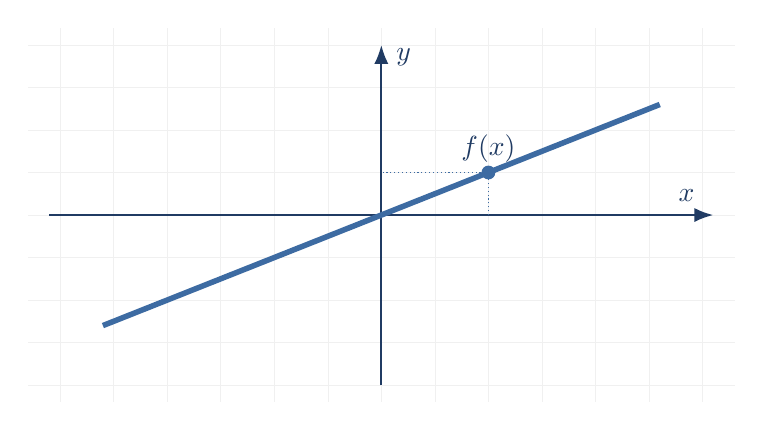
\begin{tikzpicture}[x=.68cm,y=.54cm]
 \fill[white] (-6.6,-4.4) rectangle (6.6,4.4);
 \foreach \x in {-6,...,6}{\draw[gray!12,line width=.2pt] (\x,-4.4)--(\x,4.4);}
 \foreach \y in {-4,...,4}{\draw[gray!12,line width=.2pt] (-6.6,\y)--(6.6,\y);}
 \draw[deep,-{Latex[length=2.4mm]},thick] (-6.2,0)--(6.2,0);
 \draw[deep,-{Latex[length=2.4mm]},thick] (0,-4.0)--(0,4.0);
 \draw[mid,line width=2pt] (-5.2,-2.6)--(5.2,2.6);
 \fill[mid] (2,1) circle (2.5pt);
 \draw[mid,densely dotted] (2,0)--(2,1)--(0,1);
 \node[deep,above] at (5.7,.1){$x$};
 \node[deep,right] at (.1,3.7){$y$};
 \node[deep,above] at (2,1){$f(x)$};
\end{tikzpicture}
\end{document}